%%% Lecture 1 Slides %%%

\documentclass{beamer}

%\documentclass[handout]{beamer}
%\usepackage{pgfpages}
%\pgfpagesuselayout{2 on 1}[a4paper,border shrink=5mm]
%\pgfpagesuselayout{1 on 1}[a4paper,border shrink=5mm]



\usepackage{amssymb}
\usepackage{amsmath}


\newcommand{\bs}{\boldsymbol}
\newcommand{\mb}{\mathbf}
\newcommand{\indep}{{\bot\negthickspace\negthickspace\bot}}
\newcommand{\notindep}{{\bot\negthickspace\negthickspace\bot}{\negthinspace
  \negmedspace \negthickspace \negthickspace \diagup
  \;}}
\renewcommand{\S}{\mb{S}}

%\usepackage{pdfpages}
%\pdfpagelayout{2 on 1}

\mode<presentation>
{
  \usetheme{Singapore}    %Warsaw}
  % or ...

  \setbeamercovered{transparent}
  % or whatever (possibly just delete it)
}


\usepackage[english]{babel}
% or whatever

\usepackage[latin1]{inputenc}
% or whatever

\usepackage{times}
\usepackage[T1]{fontenc}
% Or whatever. Note that the encoding and the font should match. If T1
% does not look nice, try deleting the line with the fontenc.


\title[QTM 220] % (optional, use only with long paper titles)
{QTM 220}

\subtitle
{Observational Studies with Measured Confounding} 

\date{}%[Short Occasion] % (optional)


\subject{Talks}
% This is only inserted into the PDF information catalog. Can be left
% out. 



% If you have a file called "university-logo-filename.xxx", where xxx
% is a graphic format that can be processed by latex or pdflatex,
% resp., then you can add a logo as follows:

% \pgfdeclareimage[height=0.5cm]{university-logo}{university-logo-filename}
% \logo{\pgfuseimage{university-logo}}



% Delete this, if you do not want the table of contents to pop up at
% the beginning of each subsection:

\AtBeginSection[]
{
  \begin{frame}<beamer>
    \frametitle{Outline}
    \tableofcontents[currentsection,currentsubsection]
  \end{frame}
}


\AtBeginSubsection[]
{
  \begin{frame}<beamer>
    \frametitle{Outline}
    \tableofcontents[currentsection,currentsubsection]
  \end{frame}
}


% If you wish to uncover everything in a step-wise fashion, uncomment
% the following command: 

%\beamerdefaultoverlayspecification{<+->}


\begin{document}

\begin{frame}
  \titlepage
\end{frame}

\begin{frame}
  \frametitle{Outline}
  \tableofcontents
  % You might wish to add the option [pausesections]
\end{frame}



\section{Choosing Conditioning Variables}


\frame{
\frametitle{Omitted Variable Bias}

Suppose we believe that a two variable linear model is the true model in the Washington (2008) example,
\begin{align*}
Y_i &= \beta_0 + \beta_1 Girls_i + \beta_2 Children_i + \epsilon_i
\end{align*}
but suppose that we omit the $Children$ variable from the analysis
 \begin{align*}
Y_i &= \beta_0^{*} + \beta_1^{*} Girls_i + \epsilon_i^{*}
\end{align*}

}


\frame{

If we write the model for children as the following: 
\begin{align*}
Children_i &= \gamma_0 + \gamma_1 Girls_i + \nu_i
\end{align*}
then the two explanatory variable model can be re-written as the following:


\begin{align*}
Y_i &= \beta_0 + \beta_1 Girls_i + \beta_2 Children_i + \epsilon_i \\
&= \beta_0 + \beta_1 Girls_i + \beta_2 (\gamma_0 + \gamma_1 Girls_i + \nu_i) + \epsilon_i \\
&= \underbrace{\beta_0 + \beta_2 \gamma_0}_{\beta_0^{*}} + \underbrace{(\beta_1 + \beta_2 \gamma_1)}_{\beta_1^{*}} Girls_i + \underbrace{\epsilon_i + \beta_2 \nu_i}_{\epsilon_i^{*}}
\end{align*}
%this implies that $\beta_1^{*} = (\beta_1 + \beta_2 \gamma_1)$ and $\beta_2 \gamma_1$ describes the bias due to omitting the $Children$ variable from the model. Using the 105th congress and the AAUW scores, we can see the results of this bias. In the multiple regression model, the effect of an extra girl (conditional on number of children) is estimated to increase AAUW score by almost 6 points ($\widehat{\beta}_1= 5.776$). However, if we fail to condition on the number of children, the effect of an extra girl is estimated to decrease AAUW score by almost 3 points ($\widehat{\beta}_1^{*}= -2.784$).

}

\frame{
\frametitle{Points of Potential Confusion}

Is $\beta_1^{*}$ meant to be causal? \\
 \begin{align*}
Y_i &= \beta_0^{*} + \beta_1^{*} Girls_i + \epsilon_i^{*}
\end{align*}

\pause

\vspace{.5cm}

Is $\gamma_1$ meant to be causal?
\begin{align*}
Children_i &= \gamma_0 + \gamma_1 Girls_i + \nu_i
\end{align*}

\pause

\vspace{.5cm}

If $\gamma_1$ were meant to be causal would we want to include the omitted variable?

}


\frame{
\frametitle{Some Typical Econometric Advice}



\begin{quote}
In sum, if the variable we leave out is positively correlated with the variable we include and also has itself a positive effect on the dependent variable, then our mispecified model will produce an upward-biased estimator of the effect of $X_1$ on $Y$. [Ashenfelter, Levine, and Zimmerman, p. 189]%\cite[p. 449]{Kme86}
\end{quote}

\pause



\begin{quote}
The short answer to the questions posed above is that the OLS estimates based on the equation containing too many explanatory variables will indeed be unbiased estimates of the true parameters. [Ashenfelter, Levine, and Zimmerman, p. 187]%\cite[p. 449]{Kme86}
\end{quote}


%\begin{quote}
%The conclusion, then, is that if the specification error consists of
%including some irrelevant explanatory variables in the regression
%equation, the least squares estimators of the regression coefficients
%are unbiased but not efficient.  [Kmetka 1986, p. 449]%\cite[p. 449]{Kme86}
%\end{quote}


}



\frame{
\frametitle{Directed Acyclic Graphs}

\begin{figure}[ht]
  \begin{center}
    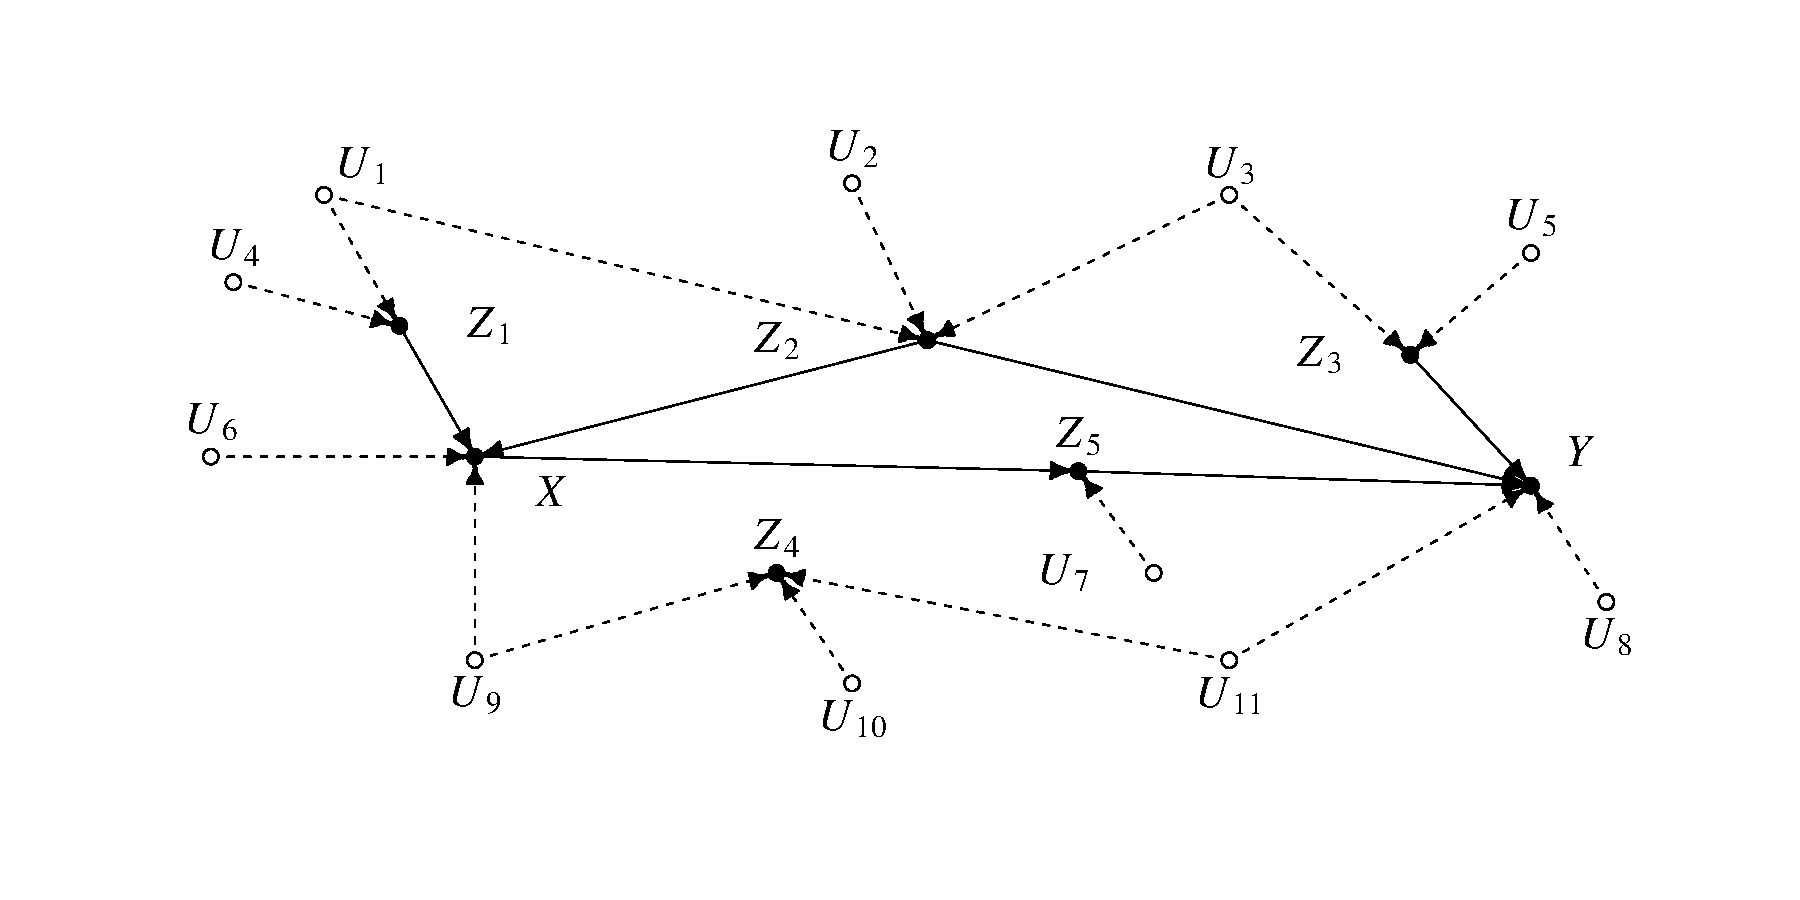
\includegraphics[width=4in,height=3in]{DAG7talk}
  \end{center}
  \vspace{-0.275in}
\end{figure}  

}


%\frame{
%\frametitle{Graphs and Potential Outcomes}

%\begin{figure}[ht]
%  \begin{center}
 %   \includegraphics[width=4in,height=3in]{DAG7subtalk}
%  \end{center}
%  \vspace{-0.275in}
%\end{figure}  

%}

%\frame{

%\begin{definition}[Effect of Action]
%Let $M$ be a causal model, $\X$ a set of variables in $\V$, and $x$ a
%particular realization of $\X$. The \emph{effect of action} $do(\X=x)$
%on $M$ is given by the submodel $M_x$. 
%\end{definition}

%\begin{definition}[Potential Outcome]
%Let $\X$ and $\Y$ be two subsets of variables in $ \V$. The
%\emph{potential outcome} of $\Y$ to action $do(\X=x)$, denoted
%$\Y_x(u)$ is the solution for $\Y$ of the set of equations $F_x$. 
%\end{definition}

%}

%\frame{
%\frametitle{Actions and Potential Outcomes}

%\begin{figure}[ht]
 % \begin{center}
  %  \includegraphics[width=4in,height=3in]{DAG7subtalk}
 % \end{center}
  %\vspace{-0.275in}
%\end{figure}  

%}




\frame{
\frametitle{Choosing Conditioning Variables}

\begin{definition}[Back-Door Criterion (Pearl (2000, p. 79))]
\begin{enumerate}
  \item none of the conditioning variables is post-$X$; and
  \item $X$ is ``$d$-separated'' from $Y$ by the conditioning variables in the graph formed by
  deleting all arrows out of $X$. 
\end{enumerate}
\end{definition}

\begin{figure}[ht]
  \begin{center}
    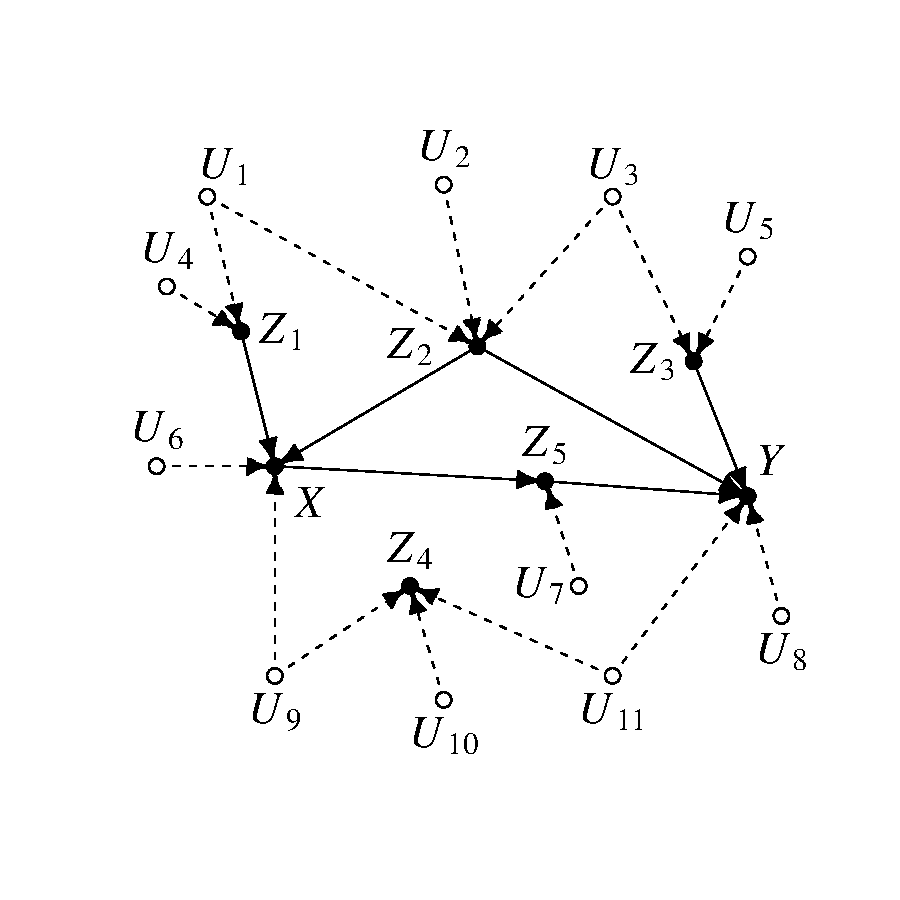
\includegraphics[width=4in,height=2in]{DAG7-full-0.pdf}
  \end{center}
  \vspace{-0.275in}
\end{figure}  
}

\frame{
\frametitle{BD1: Don't condition on post-treatment variables}

\begin{figure}[ht]
  \begin{center}
    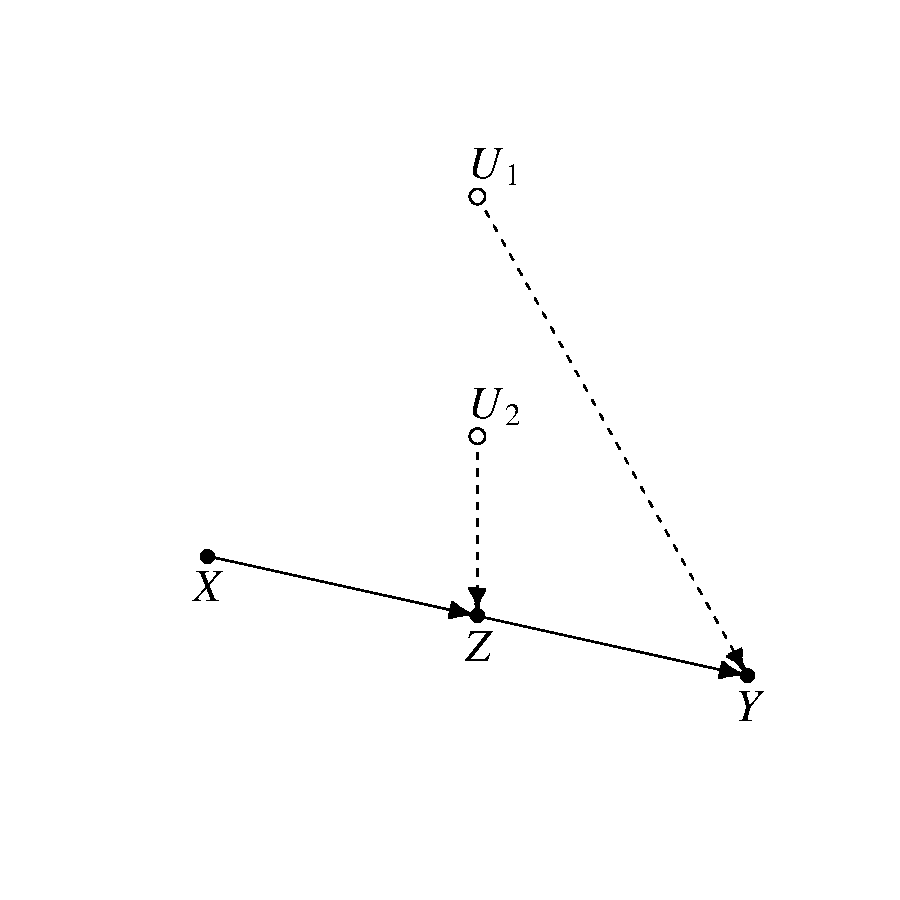
\includegraphics[width=4in,height=2in]{DAGpost0.pdf}
  \end{center}
  \vspace{-0.275in}
\end{figure}  


}

\frame{
\frametitle{BD1: Don't condition on descendants of $X$}

\begin{figure}[ht]
  \begin{center}
    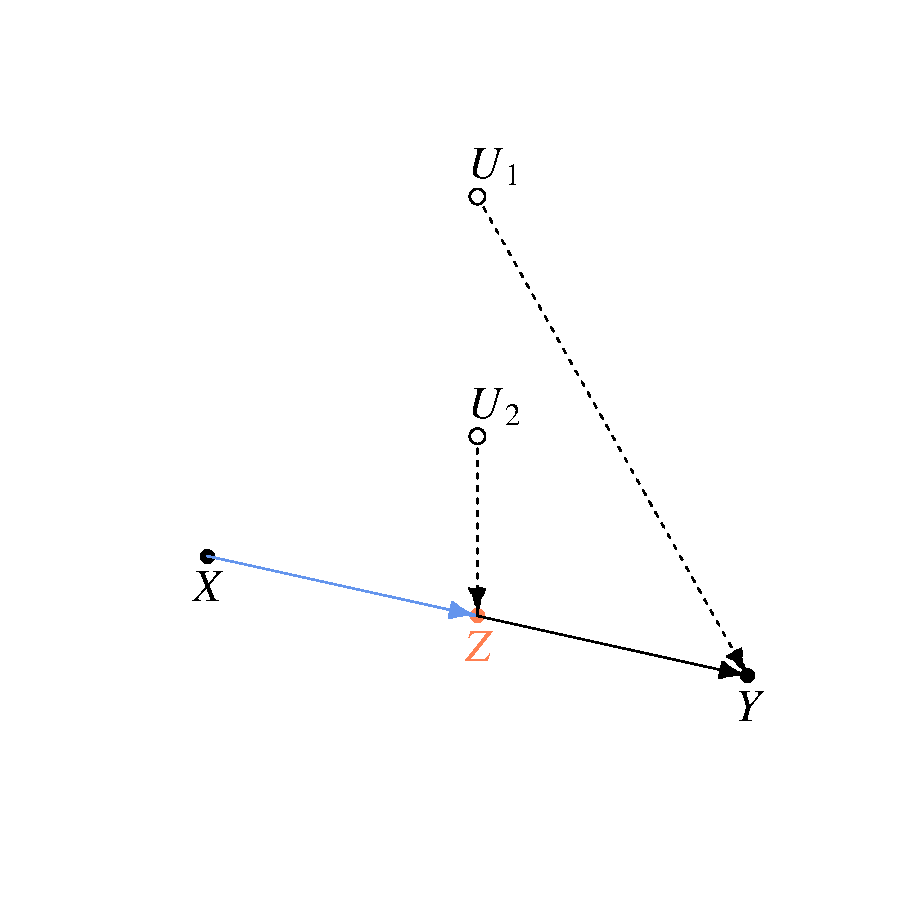
\includegraphics[width=4in,height=2in]{DAGpost1.pdf}
  \end{center}
  \vspace{-0.275in}
\end{figure}  


}

\frame{
\frametitle{BD1: Don't condition on descendants of $X$}

\begin{figure}[ht]
  \begin{center}
    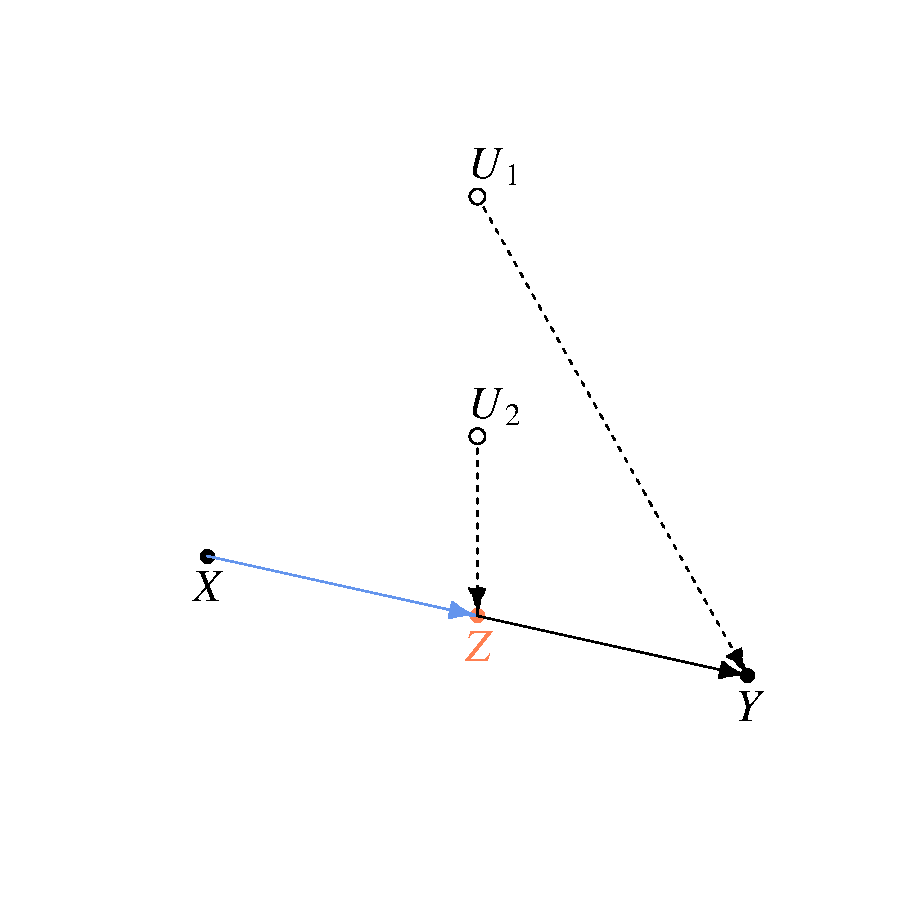
\includegraphics[width=2in,height=1in]{DAGpost1.pdf}
  \end{center}
  \vspace{-0.275in}
\end{figure}  

\begin{quote}
In sum, if the variable we leave out is positively correlated with the variable we include and also has itself a positive effect on the dependent variable, then our mispecified model will produce an upward-biased estimator of the effect of $X_1$ on $Y$. [Ashenfelter, Levine, and Zimmerman, p. 2003]%\cite[p. 449]{Kme86}
\end{quote}

}



\frame{
\frametitle{BD2: $X$ is $d$-separated from $Y$ by the conditioning variables in the graph formed by
  deleting all arrows out of $X$.}

%\begin{align*}
%P(x,y,\z,\u) &= \left( \prod_{j=1}^{11} P(u_j)\right) \cdot P(z_1|u_1,u_4) \cdot P(z_2|u_1,u_2,u_3) \\
%&\quad\quad \cdot P(z_3|u_3,u_5) \cdot P(z_4|u_9,u_{10},u_{11}) \cdot P(x|z_1,z_2,u_6,u_9) \\
%&\quad\quad \cdot P(z_5|x,u_1,u_2,u_3) \cdot P(y|z_2,z_3,z_5,u_8,u_{11}) 
%\end{align*}

\begin{definition}[$d$-Separation (Pearl (2000, p. 16))]

\begin{enumerate}
  \item $X$ is $d$-Separated from $Y$ if all paths are blocked
  \item paths are blocked by ``unconditioned colliders'' or conditioned non-colliders
\end{enumerate}
\end{definition}

\vspace{.5cm}

$d$-Separation allows conditional independence relations to be read from a DAG consistent with a probabilistic model.

}

\frame{
\frametitle{Example: Sufficient Conditioning Sets}

\begin{figure}[ht]
  \begin{center}
    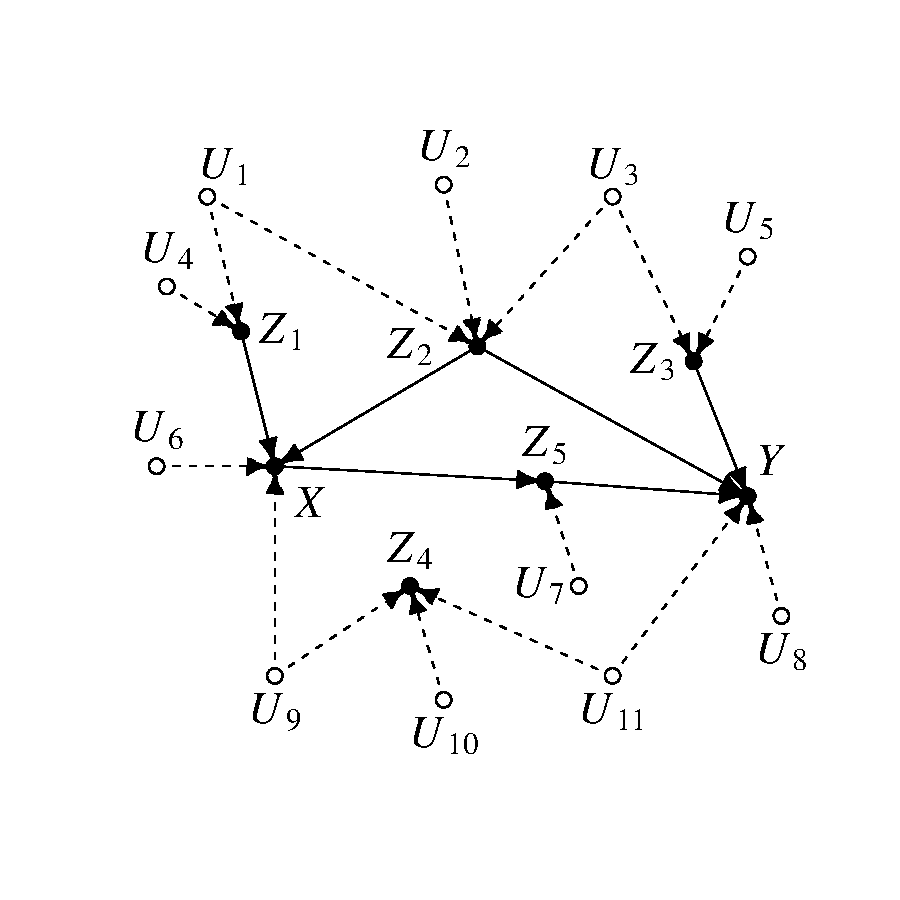
\includegraphics[width=4in,height=2in]{DAG7-full-0.pdf}
  \end{center}
  \vspace{-0.275in}
\end{figure}  

Remove arrows out of $X$. 

}

\frame{
\frametitle{Example: Sufficient Conditioning Sets}

\begin{figure}[ht]
  \begin{center}
    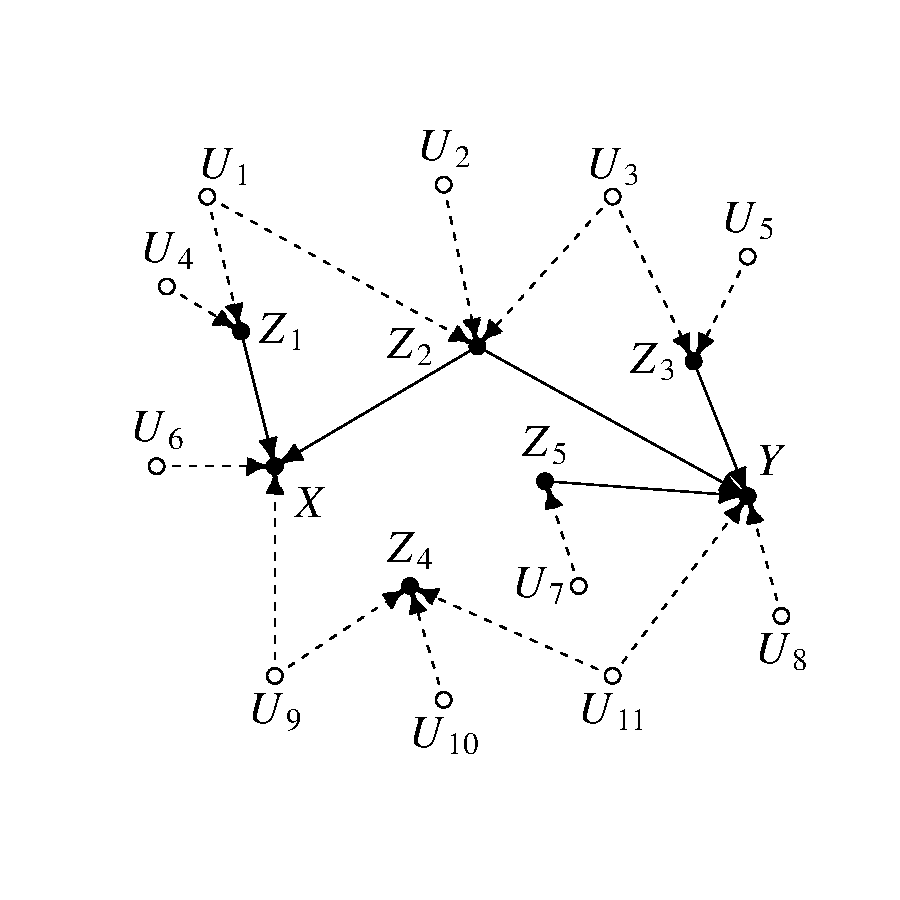
\includegraphics[width=4in,height=2in]{DAG7-nofront-0.pdf}
  \end{center}
  \vspace{-0.275in}
\end{figure}  

Recall that paths are blocked by  ``unconditioned colliders'' or conditioned non-colliders

}

\frame{
\frametitle{Example: Sufficient Conditioning Sets}

\begin{figure}[ht]
  \begin{center}
    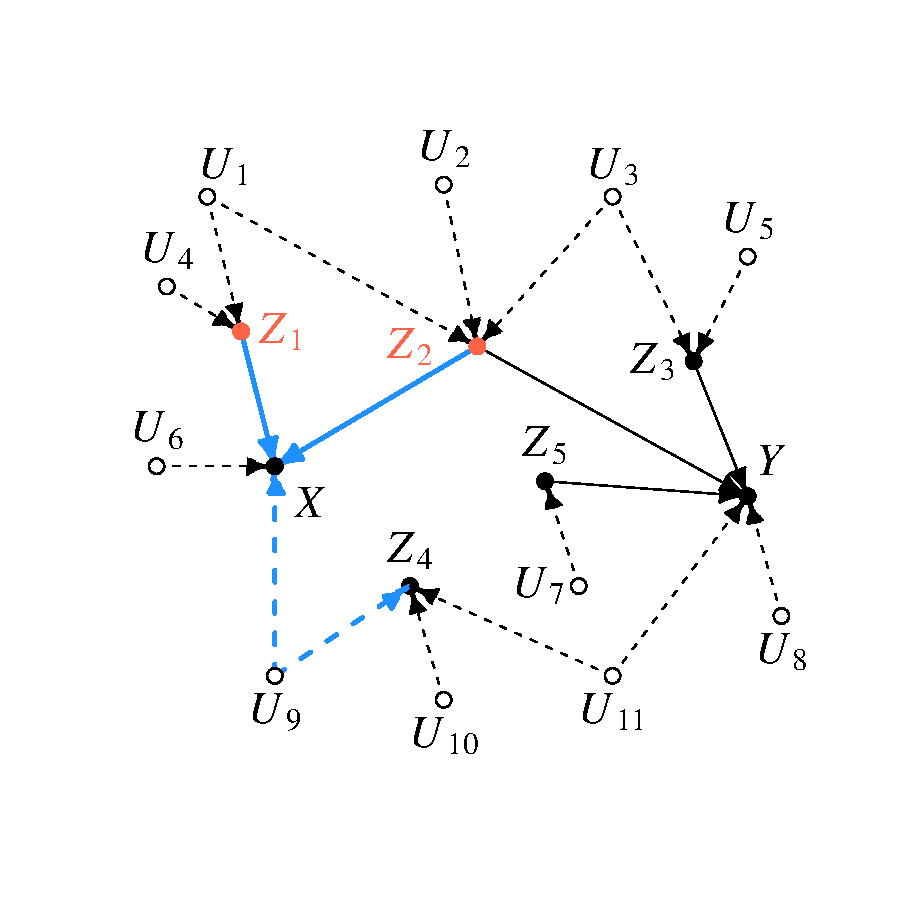
\includegraphics[width=4in,height=2in]{DAG7-nofront-1.pdf}
  \end{center}
  \vspace{-0.275in}
\end{figure}  

Recall that paths are blocked by  ``unconditioned colliders'' or conditioned non-colliders

}

\frame{
\frametitle{Example: Sufficient Conditioning Sets}

\begin{figure}[ht]
  \begin{center}
    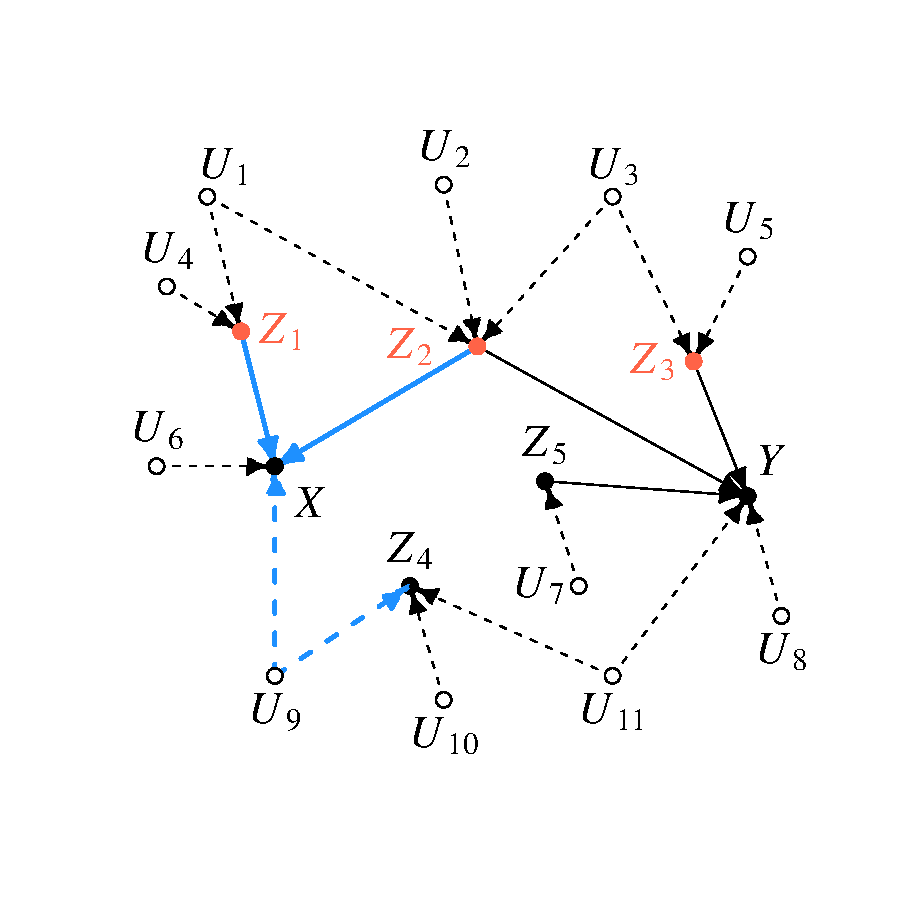
\includegraphics[width=4in,height=2in]{DAG7-nofront-2.pdf}
  \end{center}
  \vspace{-0.275in}
\end{figure}  

Recall that paths are blocked by  ``unconditioned colliders''  or conditioned non-colliders

}

\frame{
\frametitle{Example: Sufficient Conditioning Sets}

\begin{figure}[ht]
  \begin{center}
    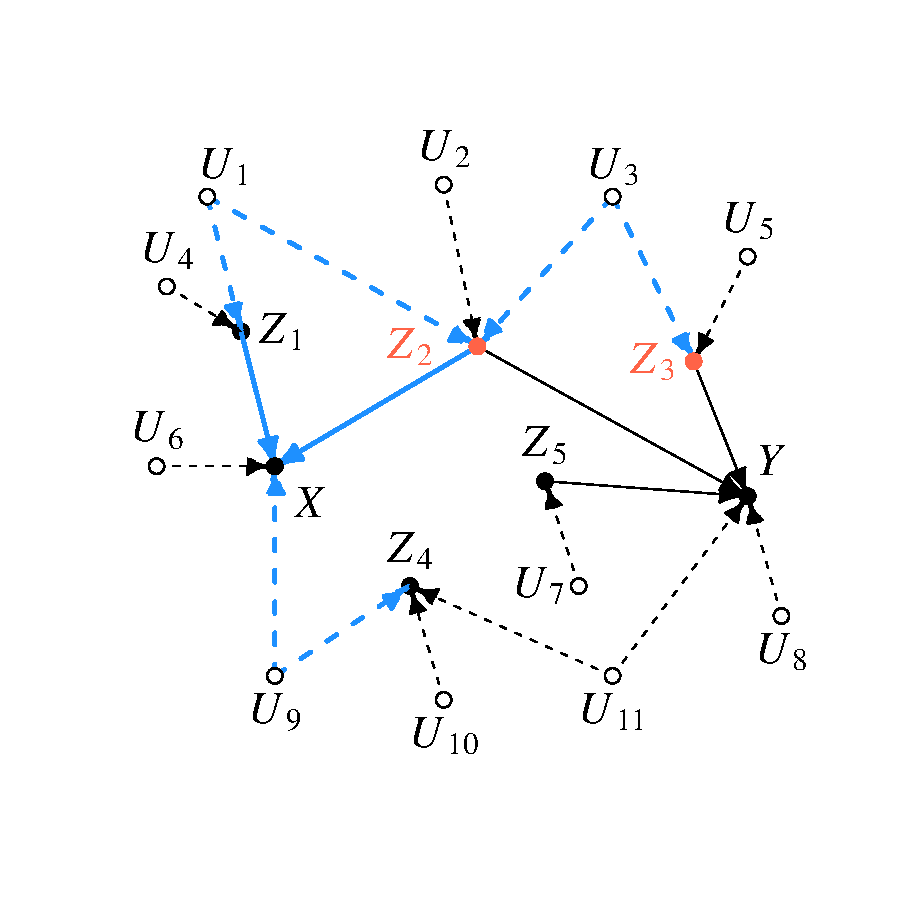
\includegraphics[width=4in,height=2in]{DAG7-nofront-3.pdf}
  \end{center}
  \vspace{-0.275in}
\end{figure}  

Recall that paths are blocked by  ``unconditioned colliders'' or conditioned non-colliders

}

\frame{
\frametitle{Example: Non-sufficient Conditioning Sets}

\begin{figure}[ht]
  \begin{center}
    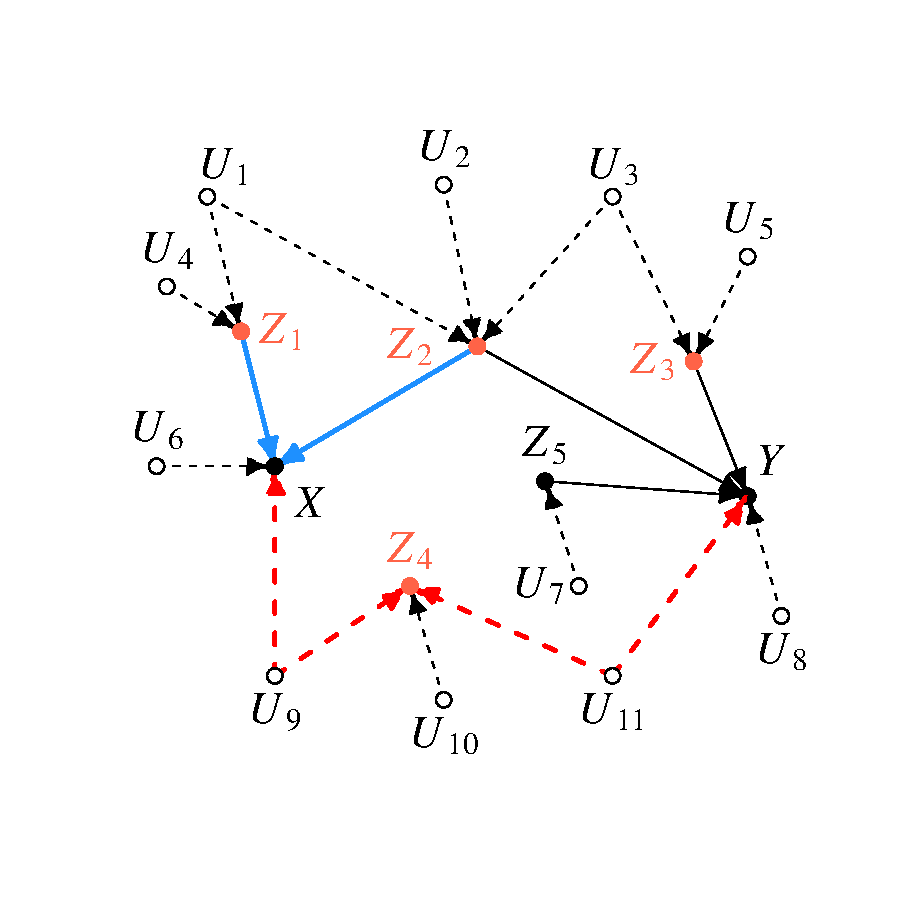
\includegraphics[width=4in,height=2in]{DAG7-nofront-4.pdf}
  \end{center}
  \vspace{-0.275in}
\end{figure}  

Recall that paths are blocked by  ``unconditioned colliders'' or conditioned non-colliders

}

\frame{
\frametitle{Example: Non-sufficient Conditioning Sets}

\begin{figure}[ht]
  \begin{center}
    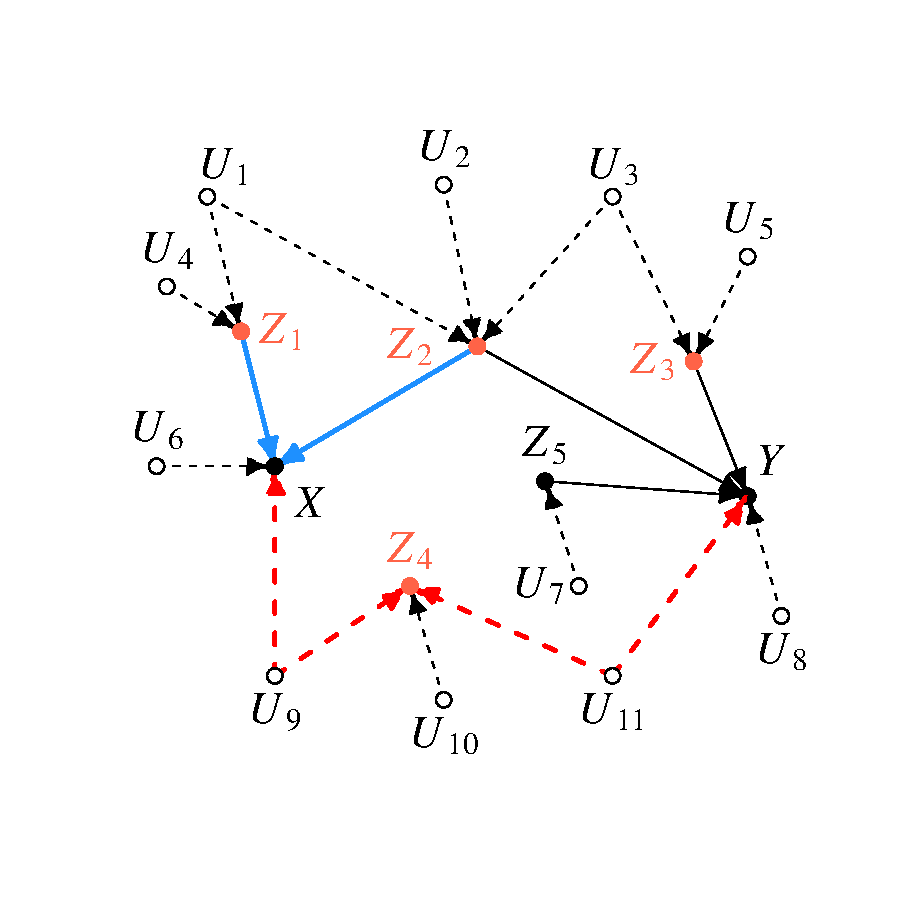
\includegraphics[width=2in,height=1in]{DAG7-nofront-4.pdf}
  \end{center}
  \vspace{-0.275in}
\end{figure}  

\begin{quote}
The short answer to the questions posed above is that the OLS estimates based on the equation containing too many explanatory variables will indeed be unbiased estimates of the true parameters. [Ashenfelter, Levine, and Zimmerman, p. 187]%\cite[p. 449]{Kme86}
\end{quote}

%\begin{quote}
%The conclusion, then, is that if the specification error consists of
%including some irrelevant explanatory variables in the regression
%equation, the least squares estimators of the regression coefficients
%are unbiased but not efficient.  [Kmetka 1986, p. 449]%\cite[p. 449]{Kme86}
%\end{quote}

}


\section{Estimation with Regression}


\frame{
\frametitle{One Child Legislators in the Washington (2008) Data}

\begin{figure}[ht]
  \begin{center}
    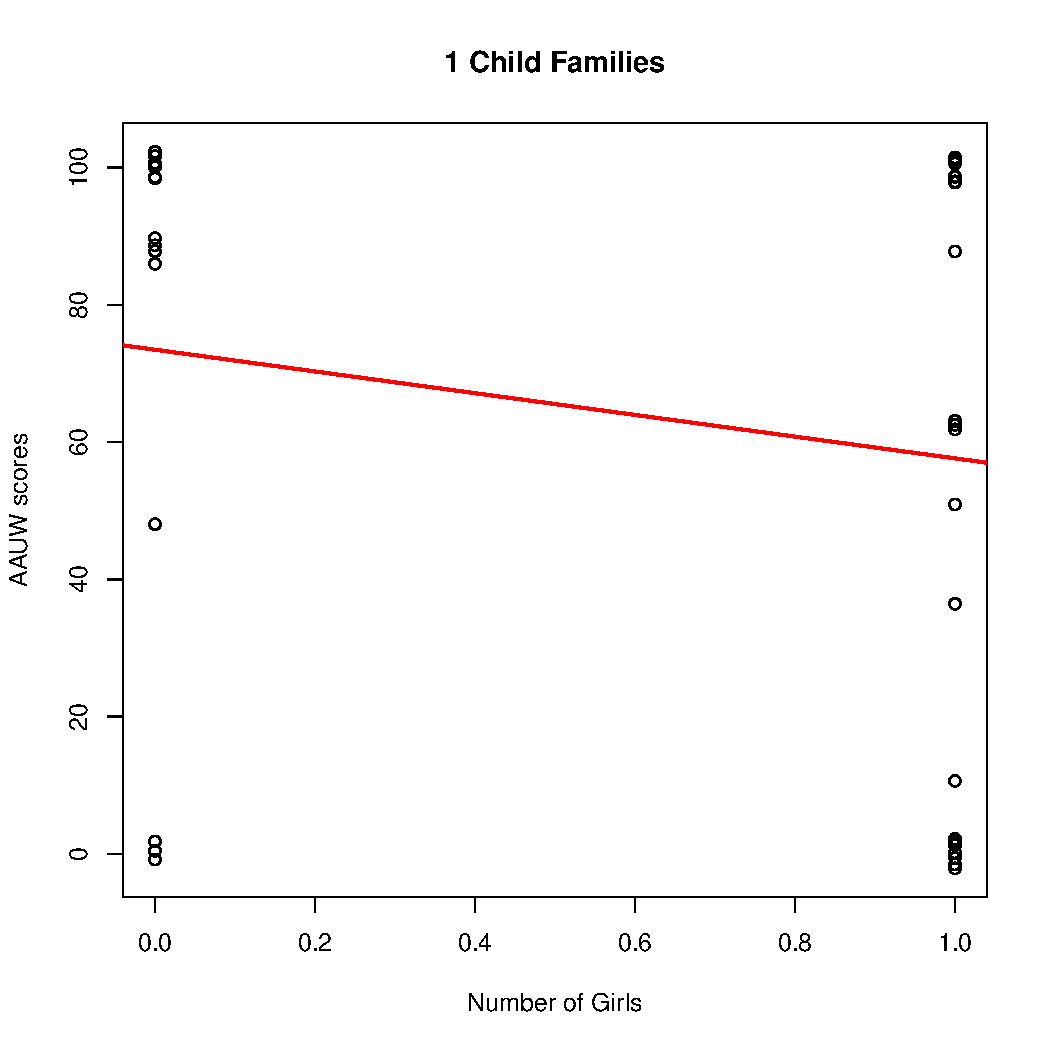
\includegraphics[height=2.5in]{1ch.pdf}
  \end{center}
  \vspace{-0.275in}
\end{figure}  
Among the subset of one-child legislators, we could adopt the standard potential outcomes approach.


}



\frame{
\frametitle{Two Children Legislators in the Washington (2008) Data}

\begin{figure}[ht]
  \begin{center}
    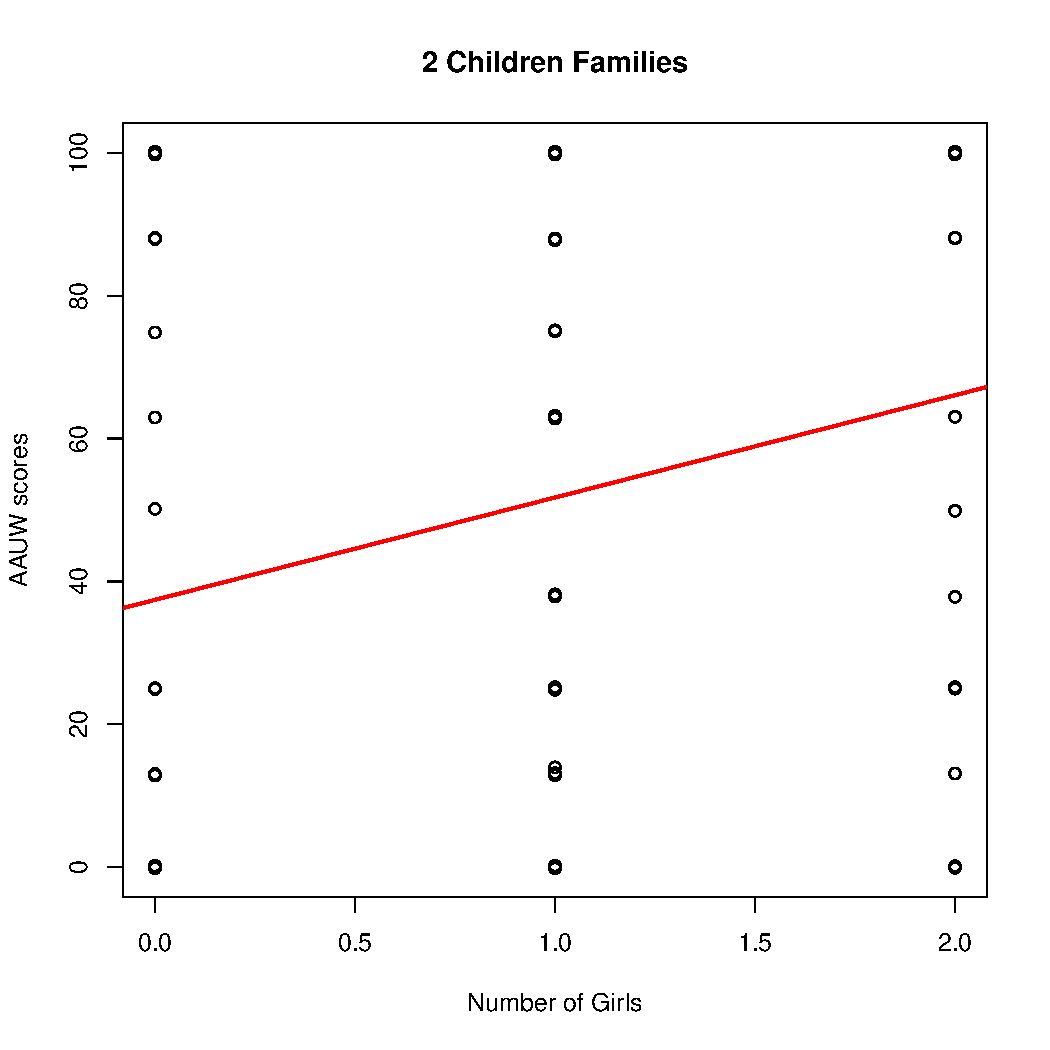
\includegraphics[height=2.5in]{2ch.pdf}
  \end{center}
  \vspace{-0.275in}
\end{figure}  
How would you construct the potential outcomes table for families with 2 children? \pause
What assumption is now implicit in the regression?

}


\frame{
Among the subset of 2 children legislators, assume a linear CEF 
\begin{align*}
E[Y|T=t] = \beta_0 + \beta_1 \cdot t 
\end{align*}
\pause
When is $\beta_1$ interpretable as the ATE of a one unit increase? 
\begin{align*}
\beta_1 &= E[Y|T=t+1]-E[Y|T=t] \text{ for all } t  \\
&=\onslide<3->{E[Y(t+1)|T=t+1]-E[Y(t)|T=t] \text{ for all } t }\\
&=\onslide<4->{E[Y(t+1)-Y(t)]  \text{ for all } t }
\end{align*}

\onslide<5->{This linear approach would also be straightforward for 3 children, 4 children, etc.}\\ 

\vspace{.5cm}

\onslide<6>{What are some ways we could combine these analyses across all legislators?}

}



\frame{
Assume a linear additive CEF
\begin{align*}
E[Y|T=t,X=x] = \beta_0 + \beta_1 \cdot t + \beta_2 \cdot x
\end{align*}
\pause

\vspace{.5cm}

When is $\beta_1$ interpretable as the ATE of a one unit increase? 
{\footnotesize
\begin{align*}
\beta_1 &= \onslide<3->{E[Y|T=t+1,X=x]-E[Y|T=t,X=x] \text{ for all } t,x} \\
&= \onslide<4->{E_X\left\{E[Y|T=t+1,X=x]-E[Y|T=t,X=x]\right\} \text{ for all } t} \\
&= \onslide<5->{E_X\left\{E[Y(t+1)|T=t+1,X=x]-E[Y(t)|T=t,X=x]\right\} \text{ for all } t} \\
&= \onslide<6->{E_X\left\{E[Y(t+1)|X=x]-E[Y(t)|X=x]\right\} \text{ for all } t} \\
&= \onslide<7->{E_X\left\{E[Y(t+1)-Y(t)|X=x]\right\} \text{ for all } t} \\
&= \onslide<8->{E[Y(t+1)-Y(t)]  \text{ for all } t} 
\end{align*}}

}

\frame{
\frametitle{The Additive Linear Model}

\begin{figure}[ht]
  \begin{center}
    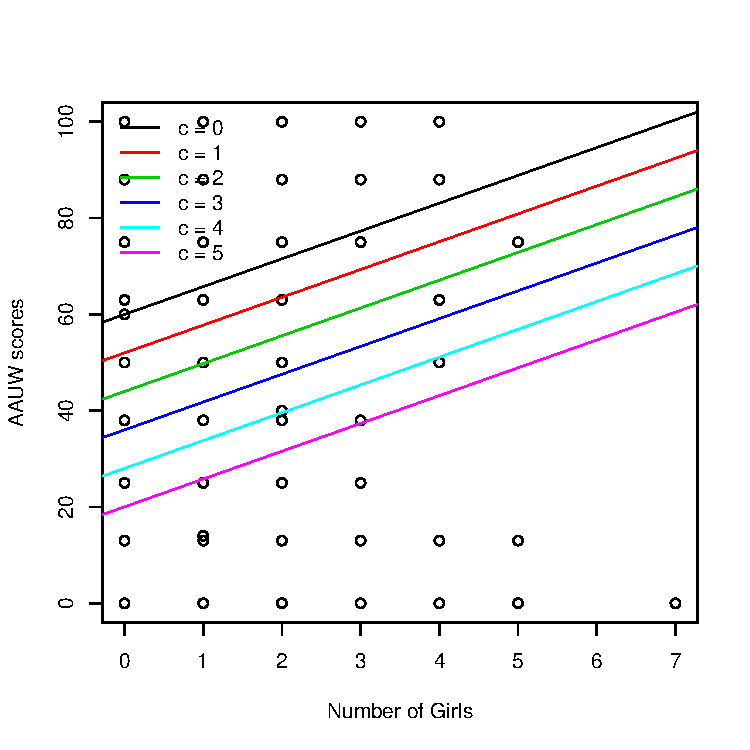
\includegraphics[height=2.5in]{3e.pdf}
  \end{center}
  \vspace{-0.275in}
\end{figure}  \pause

How would this picture change if we used the model in Equation 1 of Washington (2008)?

}

\frame{
\frametitle{The Interactive Linear Model}


\begin{align*}
E[Y|T=t,X=x] &= \onslide<1->{\beta_0 + \beta_1 \cdot t + \beta_2 \cdot x+ \beta_3 \cdot t \cdot x} \\
&= \onslide<2->{\beta_0 + \bs{(\beta_1 + \beta_3 \cdot x)} \cdot t + \beta_2 \cdot x}
\end{align*}
\onslide<2->{When is $(\beta_1 + \beta_3 \cdot x)$ interpretable as the ATE of a one unit increase, conditional on $X=x$?} 
{\footnotesize
\begin{align*}
\onslide<2->{(\beta_1 + \beta_3 \cdot x)} &\onslide<2->{=} \onslide<3->{E[Y|T=t+1,X=x]-E[Y|T=t,X=x] \text{ for all } t,x}\\
&\onslide<2->{=} \onslide<4->{E[Y|T=t+1,X=x]-E[Y|T=t,X=x] \text{ for all } t } \\
&\onslide<2->{=} \onslide<5->{E[Y(t+1)|T=t+1,X=x]-E[Y(t)|T=t,X=x] \text{ for all } t} \\
&\onslide<2->{=} \onslide<6->{E[Y(t+1)|X=x]-E[Y(t)|X=x] \text{ for all } t}  \\
&\onslide<2->{=} \onslide<7->{E[Y(t+1)-Y(t)|X=x]\ \text{ for all } t} 
\end{align*}}

}



\frame{
\frametitle{The Interactive Linear Model}

\begin{figure}[ht]
  \begin{center}
    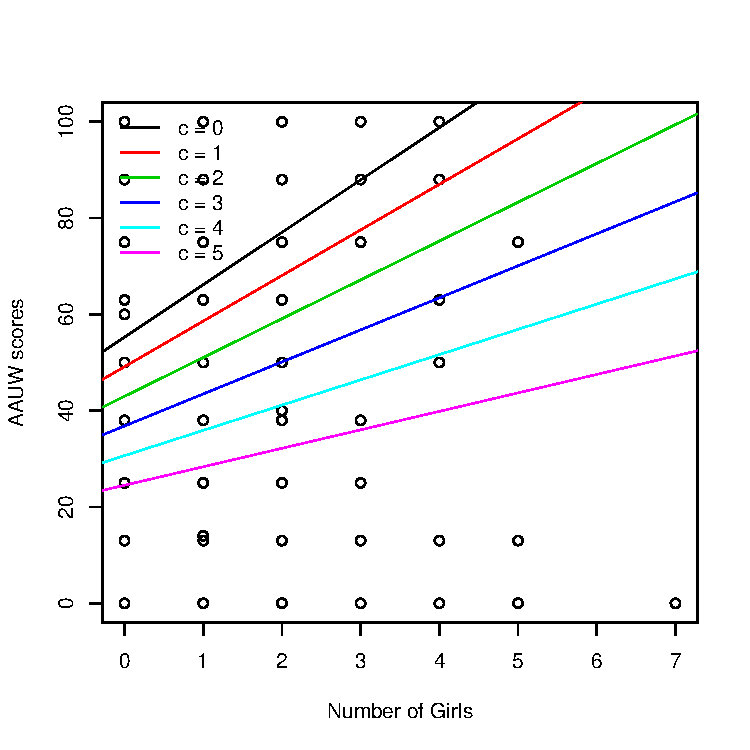
\includegraphics[height=2.5in]{3f.pdf}
  \end{center}
  \vspace{-0.275in}
\end{figure}  

 \pause

What would the picture look like if we used a more general model (for which the interactive model and Equation 1 of Washington (2008) are special cases)?



}


\frame{
\frametitle{Standardization in the Interactive Linear Model}

When is $\beta_1 + \beta_3 \cdot E_X\left\{X \right\}$ interpretable as the ATE of a one unit increase? 
\begin{align*}
\beta_1 &+ \beta_3 \cdot E_X\left\{X \right\} = \onslide<2->{E_X\left\{\beta_1 + \beta_3 \cdot X \right\}} \\
&= \onslide<3->{E_X\left\{E[Y|T=t+1,X=x]-E[Y|T=t,X=x]\right\}}\\
&= \onslide<4->{E_X\left\{E[Y(t+1)|T=t+1,X=x]-E[Y(t)|T=t,X=x]\right\}} \\
&= \onslide<5->{E_X\left\{E[Y(t+1)|X=x]-E[Y(t)|X=x]\right\}}\\
&= \onslide<6->{E_X\left\{E[Y(t+1)-Y(t)|X=x]\right\}} \\
&= \onslide<7->{E[Y(t+1)-Y(t)]} 
\end{align*}

}

\frame{
\frametitle{Standardization in the Interactive Linear Model}

\begin{figure}[ht]
  \begin{center}
    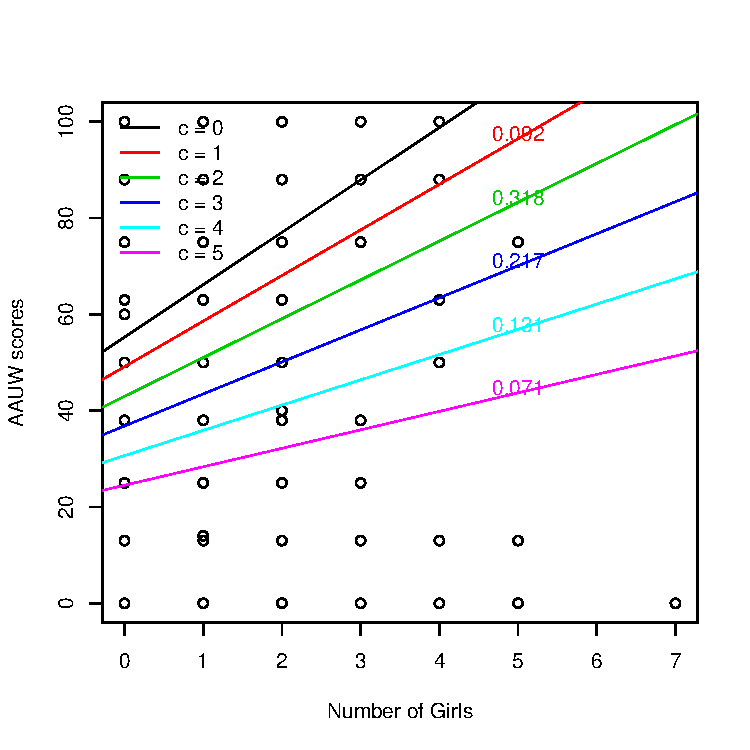
\includegraphics[height=2.5in]{3ff.pdf}
  \end{center}
  \vspace{-0.275in}
\end{figure}  


}



\frame{
\frametitle{Summary}

\begin{itemize}
\item The classical advice about choosing conditioning variables can lead to post-treatment bias or M-bias. \pause
\item Condition on ``confounding'' variables (as defined by the backdoor criterion). \pause
\item Regression can be used for causal inference, however \pause
\begin{itemize}
\item be aware of the consequences of linearity assumptions \pause
\item be aware of the consequences of additivity assumptions 
\end{itemize}
\end{itemize}

}

%\frame{
%\frametitle{Next Week}
%
%Observational Studies with Measured Confounding
%
%\begin{itemize}
%\item Assessing Overlap and Balance 
%\item Revising the Question of Interest 
%\item Relaxing Linearity and Additivity
%\item Bounding and Sensitivity Analysis for Unmeasured Confounding
%\end{itemize}
%
%\vspace{.5cm}
%
%Things to do:
%\begin{itemize}
%\item problem set 
%\item the reading and the reading quiz (see updated syllabus)
%\item annotations
%\end{itemize}
%
%
%}
%
%
\end{document}




%%%%%%%%%%%%%%%%%%%%%%%%%%%%%%

